\documentclass[letterpaper, 9pt]{extarticle}
% \usepackage{fontspec}

% ==================================================

% document parameters
% \usepackage[spanish, mexico, es-lcroman]{babel}
\usepackage[english]{babel}
\usepackage[margin=2cm]{geometry}

% ==================================================

% Packages for math
\usepackage{mathrsfs}
\usepackage{amsfonts}
\usepackage{amsmath}
\usepackage{amsthm}
\usepackage{amssymb}
\usepackage{physics}
\usepackage{dsfont}
\usepackage{esint}

% ==================================================

% Packages for writing
\usepackage{enumerate}
\usepackage[shortlabels]{enumitem}
\usepackage{framed}
\usepackage{csquotes}
\usepackage{gensymb}

% ==================================================

% Miscellaneous packages
\usepackage{float}
\usepackage{tabularx}
\usepackage{xcolor}
\usepackage{multicol}
\usepackage{subcaption}
\usepackage{caption}
\usepackage{graphicx}
\usepackage{array}
\usepackage{circuitikz}
\captionsetup{format = hang, margin = 10pt, font = small, labelfont = bf}
\usepackage{pgfplots} 

% Citation
\usepackage[round, authoryear]{natbib}

% Hyperlinks setup
\usepackage{hyperref}
\definecolor{links}{rgb}{0.36,0.54,0.66}
\hypersetup{
   colorlinks = true,
    linkcolor = black,
     urlcolor = blue,
    citecolor = blue,
    filecolor = blue,
    pdfauthor = {Author},
     pdftitle = {Title},
   pdfsubject = {subject},
  pdfkeywords = {one, two},
  pdfproducer = {LaTeX},
   pdfcreator = {pdfLaTeX},
   }

\usepackage{titlesec}
\usepackage[many]{tcolorbox}

% Adjust spacing after the chapter title
\titlespacing*{\chapter}{0cm}{-2.0cm}{0.50cm}
\titlespacing*{\section}{0cm}{0.50cm}{0.25cm}

% Indent 
\setlength{\parindent}{0pt}
\setlength{\parskip}{1ex}

% --- Theorems, lemma, corollary, postulate, definition ---
% \numberwithin{equation}{section}

\newtcbtheorem[]{problem}{Problem}%
    {enhanced,
    colback = black!5, %white,
    colbacktitle = black!5,
    coltitle = black,
    boxrule = 0pt,
    frame hidden,
    borderline west = {0.5mm}{0.0mm}{black},
    fonttitle = \bfseries\sffamily,
    breakable,
    before skip = 3ex,
    after skip = 3ex
}{problem}

\tcbuselibrary{skins, breakable}

% --- You can define your own color box. Just copy the previous \newtcbtheorm definition and use the colors of yout liking and the title you want to use.
% --- Basic commands ---
%   Euler's constant
\newcommand{\eu}{\mathrm{e}}

%   Imaginary unit
\newcommand{\im}{\mathrm{i}}

%   Sexagesimal degree symbol
\newcommand{\grado}{\,^{\circ}}

% --- Comandos para álgebra lineal ---
% Matrix transpose
\newcommand{\transpose}[1]{{#1}^{\mathsf{T}}}

%%% Comandos para cálculo
%   Definite integral from -\infty to +\infty
\newcommand{\Int}{\int\limits_{-\infty}^{\infty}}

%   Indefinite integral
\newcommand{\rint}[2]{\int{#1}\dd{#2}}

%  Definite integral
\newcommand{\Rint}[4]{\int\limits_{#1}^{#2}{#3}\dd{#4}}

%   Dot product symbol (use the command \bigcdot)
\makeatletter
\newcommand*\bigcdot{\mathpalette\bigcdot@{.5}}
\newcommand*\bigcdot@[2]{\mathbin{\vcenter{\hbox{\scalebox{#2}{$\m@th#1\bullet$}}}}}
\makeatother

%   Hamiltonian
\newcommand{\Ham}{\hat{\mathcal{H}}}

%   Trace
\renewcommand{\Tr}{\mathrm{Tr}}

% Christoffel symbol of the second kind
\newcommand{\christoffelsecond}[4]{\dfrac{1}{2}g^{#3 #4}(\partial_{#1} g_{#2 #4} + \partial_{#2} g_{#1 #4} - \partial_{#4} g_{#1 #2})}

% Riemann curvature tensor
\newcommand{\riemanncurvature}[5]{\partial_{#3} \Gamma_{#4 #2}^{#1} - \partial_{#4} \Gamma_{#3 #2}^{#1} + \Gamma_{#3 #5}^{#1} \Gamma_{#4 #2}^{#5} - \Gamma_{#4 #5}^{#1} \Gamma_{#3 #2}^{#5}}

% Covariant Riemann curvature tensor
\newcommand{\covariantriemanncurvature}[5]{g_{#1 #5} R^{#5}{}_{#2 #3 #4}}

% Ricci tensor
\newcommand{\riccitensor}[5]{g_{#1 #5} R^{#5}{}_{#2 #3 #4}}
\begin{document}
\setlist{itemsep=.5em}
\begin{Huge}
\textsf{\textbf{Fisica 2 (Teoria dei Circuiti)}}\\
Esperienza 2
\end{Huge}

\vspace{1ex}

\textsf{\textbf{Studenti:}} \text{Angelo Perotti},  \text{Mattia Zagatti}, \text{Mattia Dolci}

\vspace{2ex}

\section{Introduzione}
Lo scopo di questa seconda esperienza di laboratorio è stato acquisire dimestichezza con strumenti essenziali del Laboratorio di Elettronica, in particolare con il generatore di forme d’onda e l’oscilloscopio. Durante questa sessione, abbiamo analizzato il comportamento del circuito RC, osservandone la risposta a diverse frequenze e forme d’onda. Attraverso l’utilizzo dell’oscilloscopio, siamo stati in grado di visualizzare e misurare l’andamento temporale delle tensioni e delle correnti nel circuito RC.

\section{Materiale utilizzato}
\begin{itemize}
    \item \textbf{Componenti elettronici}: resistori (\(1 \, \text{k}\Omega\), \(10 \, \text{k}\Omega\), \(100 \, \text{k}\Omega\)), capacitori (\(10 \text{nF}\), \(100\text{nF}\)), breadboard.
    \item \textbf{Strumenti di misura}: generatore di forme d'onda, oscilloscopio
    \item \textbf{Cavi}: cavi bnc, cavi banana-banana, cavi jumper.
\end{itemize}

\section{Circuito RC}
\begin{figure}[!ht]
\centering
\resizebox{0.50\textwidth}{!}{%
\begin{circuitikz}
\tikzstyle{every node}=[font=\LARGE]
\draw (8.75,17.5) to[R] (11.25,17.5);
\draw (8.75,17.5) to[sinusoidal voltage source, sources/symbol/rotate=auto] (8.75,16.25);
\draw (11.25,17.5) to[C] (11.25,16.25);
\draw (8.75,16.25) to[short] (11.25,16.25);
\draw (11.25,17.5) to[short, -o] (12.5,17.5) ;
\draw (11.25,16.25) to[short, -o] (12.5,16.25) ;
\node [font=\LARGE] at (7.35,16.90) {$V_{in}(t)^+_-$};
\node [font=\LARGE] at (10,18) {R};
\node [font=\LARGE] at (10.53,16.85) {C};
\node [font=\LARGE] at (12.85,17.5) {+};
\node [font=\LARGE] at (12.85,16.25) {-};
\node [font=\LARGE] at (12.85,16.85) {$V_{out}(t)$};
\end{circuitikz}
}%
\caption{Circuito RC}
\end{figure}

\section{Esperimento 1: Carica e scarica circuito RC}

Nell’esercizio in questione lo scopo è quello di verificare il comportamento del circuito RC, variando i valori di resistenza e di capacità. Esso è composto da tre elementi fondamentali: il resistore R, il condensatore C e un segnale ad onda quadra con frequenza f = 10Hz, tensione picco-picco pari a 5 V e offset pari a 2.5 V, realizzato tramite un generatore di segnali. 
In un circuito RC, la costante di tempo è pari a: 
$$\tau = RC $$
In questo caso, variando i valori di resistenza e capacità, essa rimane sempre uguale a 1 ms. Questo perché avendo un segnale d’ingresso con frequenza 10 Hz, e quindi di periodo T = 100 ms (f = 1/T), il condensatore ha modo di caricarsi in quanto ha un valore di tau molto inferiore rispetto al periodo in questione, riducendo al minimo le distorsioni del segnale misurato in uscita.

\newpage

\begin{figure}[ht]
\centering
\begin{minipage}{0.5\textwidth}
\centering
\vspace{0pt}
    \centering
    \begin{tabular}{c|c|c}
        * & x & y(V) \\
        \hline
        1 & 0 & 4,97 \\
        \hline
        2 & 500$\mu$s & 3,06 \\
        \hline
        3 & 1ms & 2,03\\
        \hline
        4 & 1,5ms & 1,36\\
        \hline
        5 & 2ms & 0,944\\
        \hline
        6 & 2,5ms & 0,663\\
        \hline
        7 & 3ms & 0,462\\
        \hline
        8 & 4ms & 0,221\\
        \hline
        9 & 5ms & 0,127\\
        \hline
        10 & 6ms & 0,06\\
        \hline
        11 & 7ms & 0,02\\
    \end{tabular}
    \caption{$R=10k\ohm$ e $100nF$}
    \label{tab:my_label}

\label{fig:my_label}
\end{minipage}%
\begin{minipage}{0.5\textwidth}
\centering
\vspace{0pt}
 \begin{tabular}{c|c|c}
        * & x & y(V) \\
        \hline
        1 & 0 & 4,18 \\
        \hline
        2 & 500$\mu$s & 2,31 \\
        \hline
        3 & 1ms & 1,28\\
        \hline
        4 & 1,5ms & 0,721\\
        \hline
        5 & 2ms & 0,382\\
        \hline
        6 & 2,5ms & 0,221\\
        \hline
        7 & 3ms & 0,118\\
        \hline
        8 & 4ms & 0,2\\
        \hline
        9 & 5ms & 0,2\\
        \hline
        10 & 6ms & /\\
        \hline
        11 & 7ms & /\\
 \end{tabular}
 \caption{$R=200k\ohm$ e $C=5nF$}
 \end{minipage}
\end{figure}

Nelle tabelle viene misurata la distanza in secondi tra segnale di ingresso e di uscita e il valore di tensione ai capi del condensatore nel tempo, dove vengono utilizzate rispettivamente nella prima $R = 10 k\ohm$ e $C = 100 nF$, mentre nella seconda $R = 200 k\ohm$ e $C = 5 nF$. Le misure vengono effettuate attraverso un oscilloscopio collegato al circuito mediante cavi di tipo bnc, spostando ogni volta gli appositi cursori. 
Come è possibile notare dai dati raccolti, il valore di tensione diminuisce col passare del tempo in quanto il condensatore si sta scaricando. Nella seconda tabella si nota come il valore di tensione in uscita sia inferiore rispetto al precedente, ciò è dovuto ad un maggior valore di resistenza di $R$ che si va a sommare alla resistenza interna dell’oscilloscopio, andando a creare l’effetto partitore e diminuendo così la tensione di uscita.

\section{Esperimento 2: Risposta all’impulso del circuito RC}
In questo esercizio si utilizza lo stesso circuito usato in precedenza, impostando però come segnale di ingresso un impulso di durata variabile ($100 \mu s$, $50 \mu s$ e $10 \mu s$) avente sempre frequenza $10Hz$, ampiezza picco-picco $Vpp = 5V$ e offset pari a $2.5V$.
\begin{figure}[ht]
    \begin{minipage}{0.33\textwidth}
    \vspace{0pt}
        \centering
        \begin{tabular}{c|c|c}
            * & x & y(V) \\
            \hline
            1 & 0 & 0,43 \\
            \hline
            2 & 500$\mu$s & 0,26 \\
            \hline
            3 & 1ms & 0,16 \\
            \hline
            4 & 1,5ms & 0,103 \\
            \hline
            5 & 2ms & 0,064 \\
            \hline
            6 & 2,5ms & 0,039 \\
            \hline
            7 & 3ms & 0,024 \\
            \hline
            8 & 4ms & 0,006 \\
            \hline
            9 & 5ms & 0,000 \\
        \end{tabular}
        \caption{Impulso di durata $100\mu s$}
    \end{minipage}%
    \begin{minipage}{0.33\textwidth}
        \centering
        \begin{tabular}{c|c|c}
            * & x & y(V) \\
            \hline
            1 & 0 & 0,225 \\
            \hline
            2 & 500$\mu$s & 0,131 \\
            \hline
            3 & 1ms & 0,080 \\
            \hline
            4 & 1,5ms & 0,048 \\
            \hline
            5 & 2ms & 0,028 \\
            \hline
            6 & 2,5ms & 0,016 \\
            \hline
            7 & 3ms & 0,008 \\
            \hline
            8 & 4ms & 0,001\\
            \hline
            9 & 5ms & / \\
        \end{tabular}
        \caption{Impulso di durata $50\mu s$}
    \end{minipage}%
    \begin{minipage}{0.33\textwidth}
        \centering
        \begin{tabular}{c|c|c}
            * & x & y(V) \\
            \hline
            1 & 0 & 0,43 \\
            \hline
            2 & 500$\mu$s & 0,22 \\
            \hline
            3 & 1ms & 0,011 \\
            \hline
            4 & 1,5ms & 0,0047 \\
            \hline
            5 & 2ms & 0,002 \\
            \hline
            6 & 2,5ms & 0,0007 \\
            \hline
            7 & 3ms & -5,1 \\
            \hline
            8 & 4ms & -6 \\
            \hline
            9 & 5ms & / \\
        \end{tabular}
        \caption{Impulso di durata $10\mu s$}
    \end{minipage}
\end{figure}
\newline
Come nell’esercizio precedente, anche in questo caso è stata misurata la distanza tra i due segnali e il valore di tensione in uscita, variando la durata dell’impulso in ingresso. Osservando i dati ricavati, è possibile notare la natura esponenziale relativa alla scarica del capacitore:
$$V(t) = V_0 e^{-Tt/RC}$$
\newpage
\begin{figure}
    \centering
    \begin{minipage}[t]{0.32\linewidth}
        \centering
        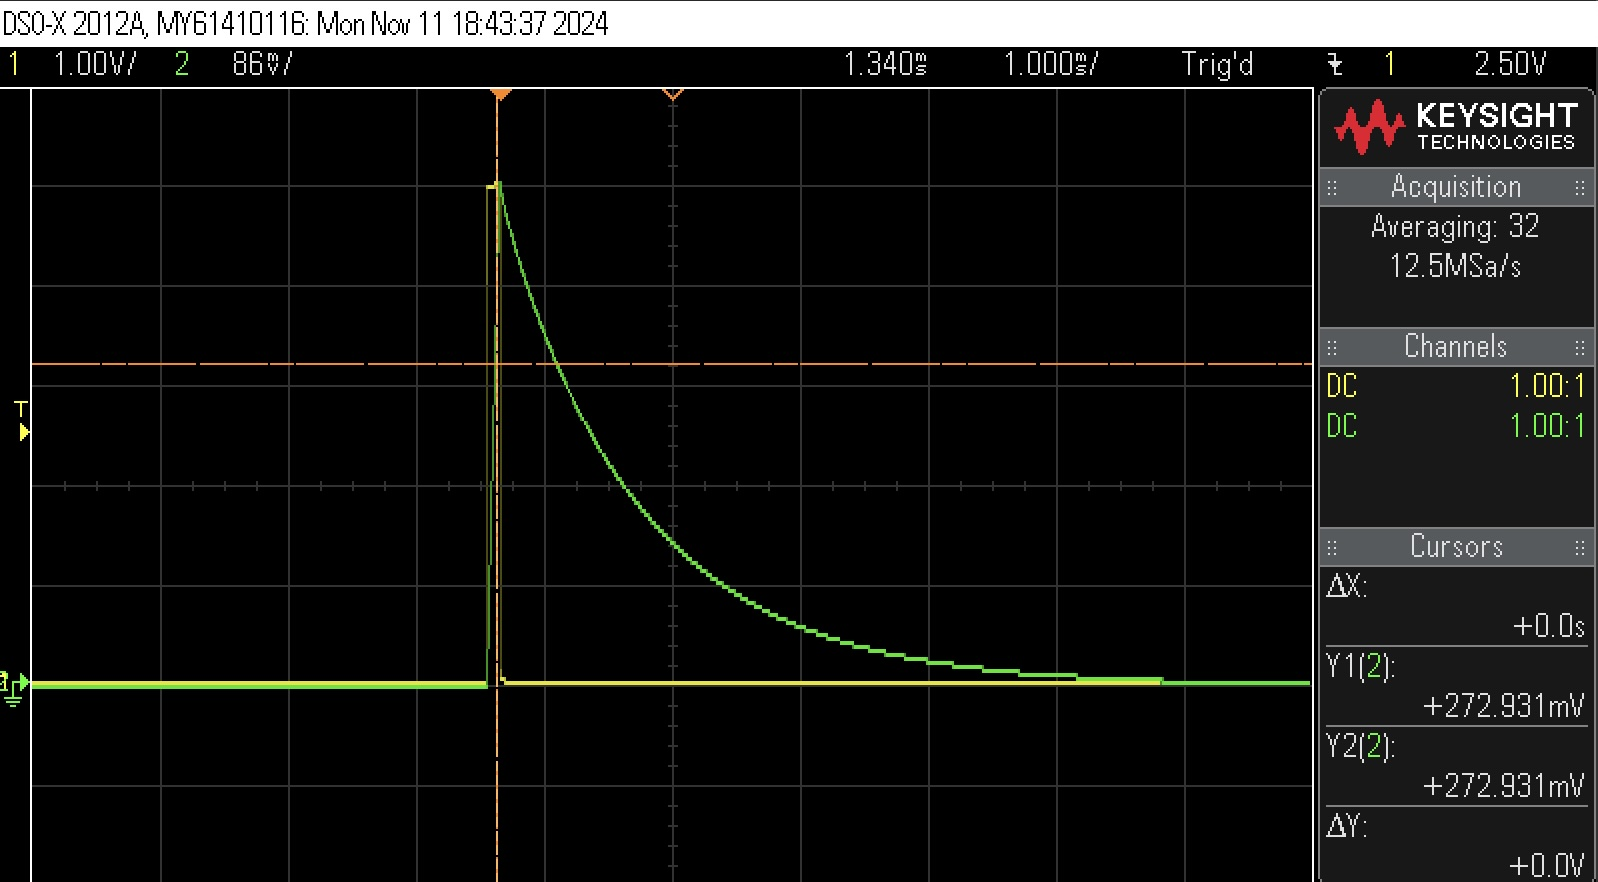
\includegraphics[width=\linewidth]{sessoesamba.jpg}
        \caption{Impulso di durata $100\mu s$}
    \end{minipage}%
    \hfill
    \begin{minipage}[t]{0.32\linewidth}
        \centering
        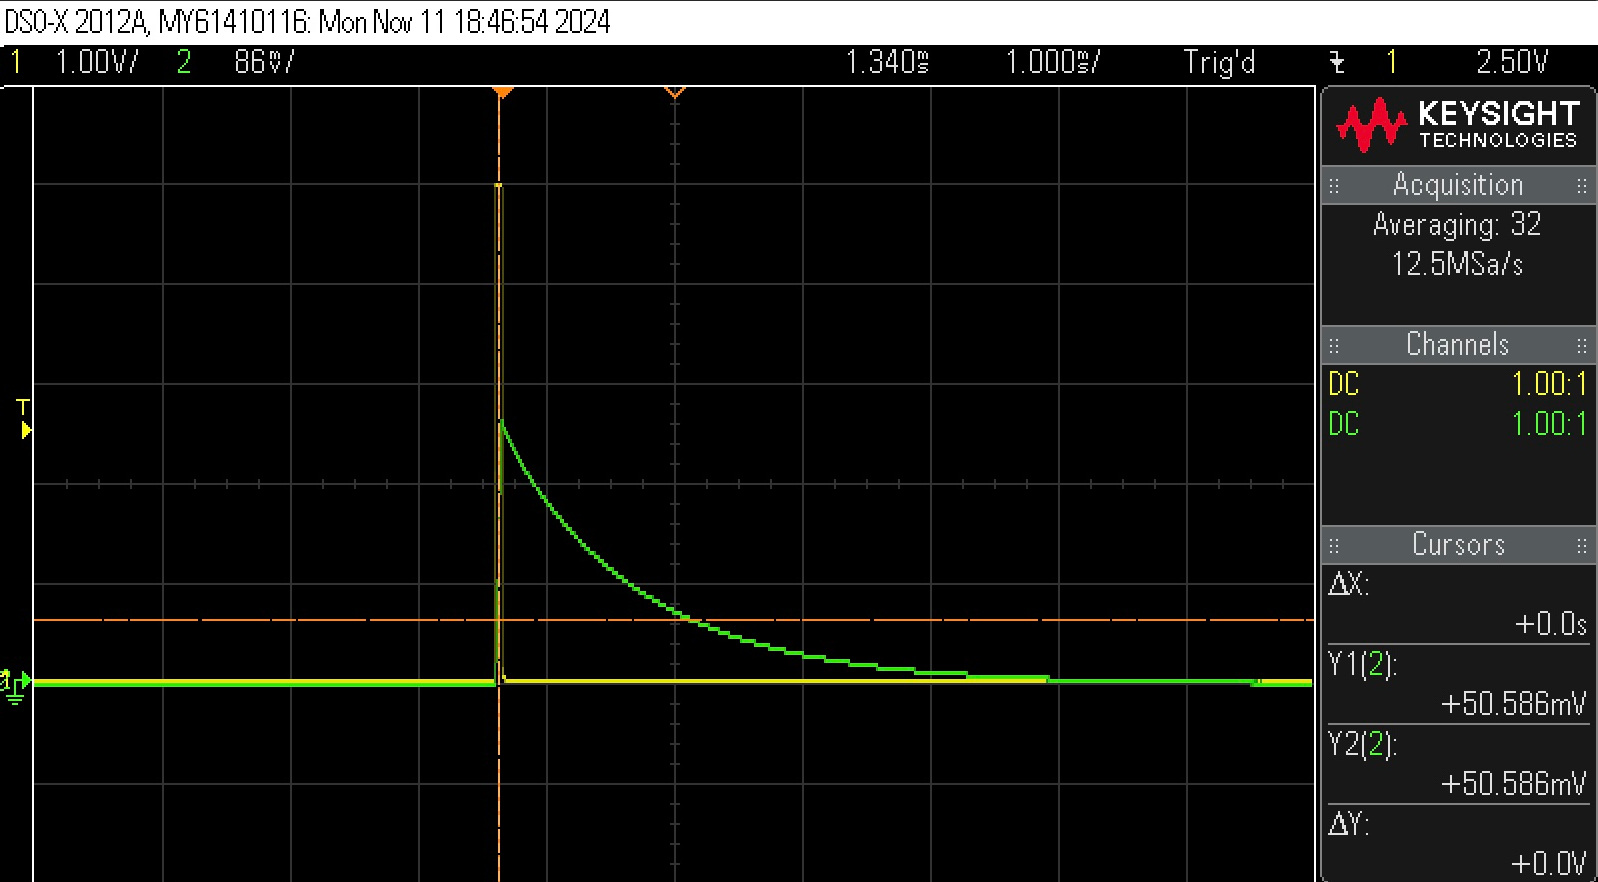
\includegraphics[width=\linewidth]{sessoesamba2.jpg}
        \caption{Impulso di durata $50\mu s$}
    \end{minipage}%
    \hfill
    \begin{minipage}[t]{0.32\linewidth}
        \centering
        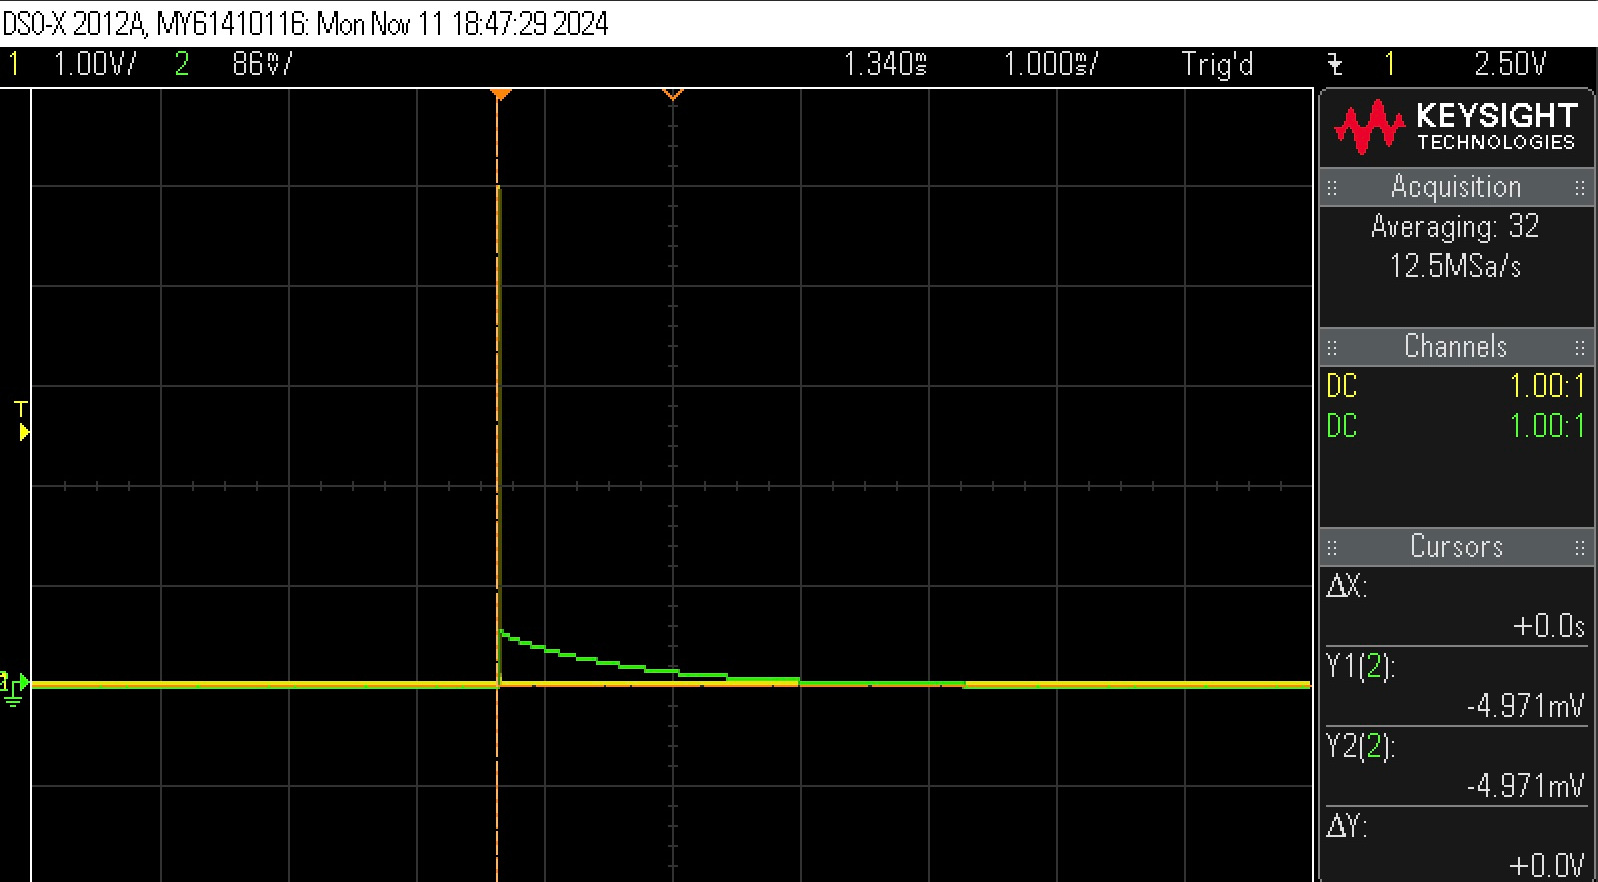
\includegraphics[width=\linewidth]{sessoesamba3.jpg}
        \caption{Impulso di durata $10\mu s$}
    \end{minipage}
\end{figure}


Le tre immagini rappresentano il segnale di uscita (segnale verde) e il segnale impulsivo di ingresso (segnale giallo), rispettivamente di durata $100 \mu s$, $50 \mu s$ e $10 \mu s$, visualizzati sull’oscilloscopio. Osservandole, è possibile notare come il valore dell’impulso più adatto per misurare la risposta del circuito è quello di $100 \mu s$ in quanto esso, rispetto agli altri due, si avvicina di più alla costante di tempo $\tau$ pari a $1 ms$.

\begin{figure}[h]
    \centering
    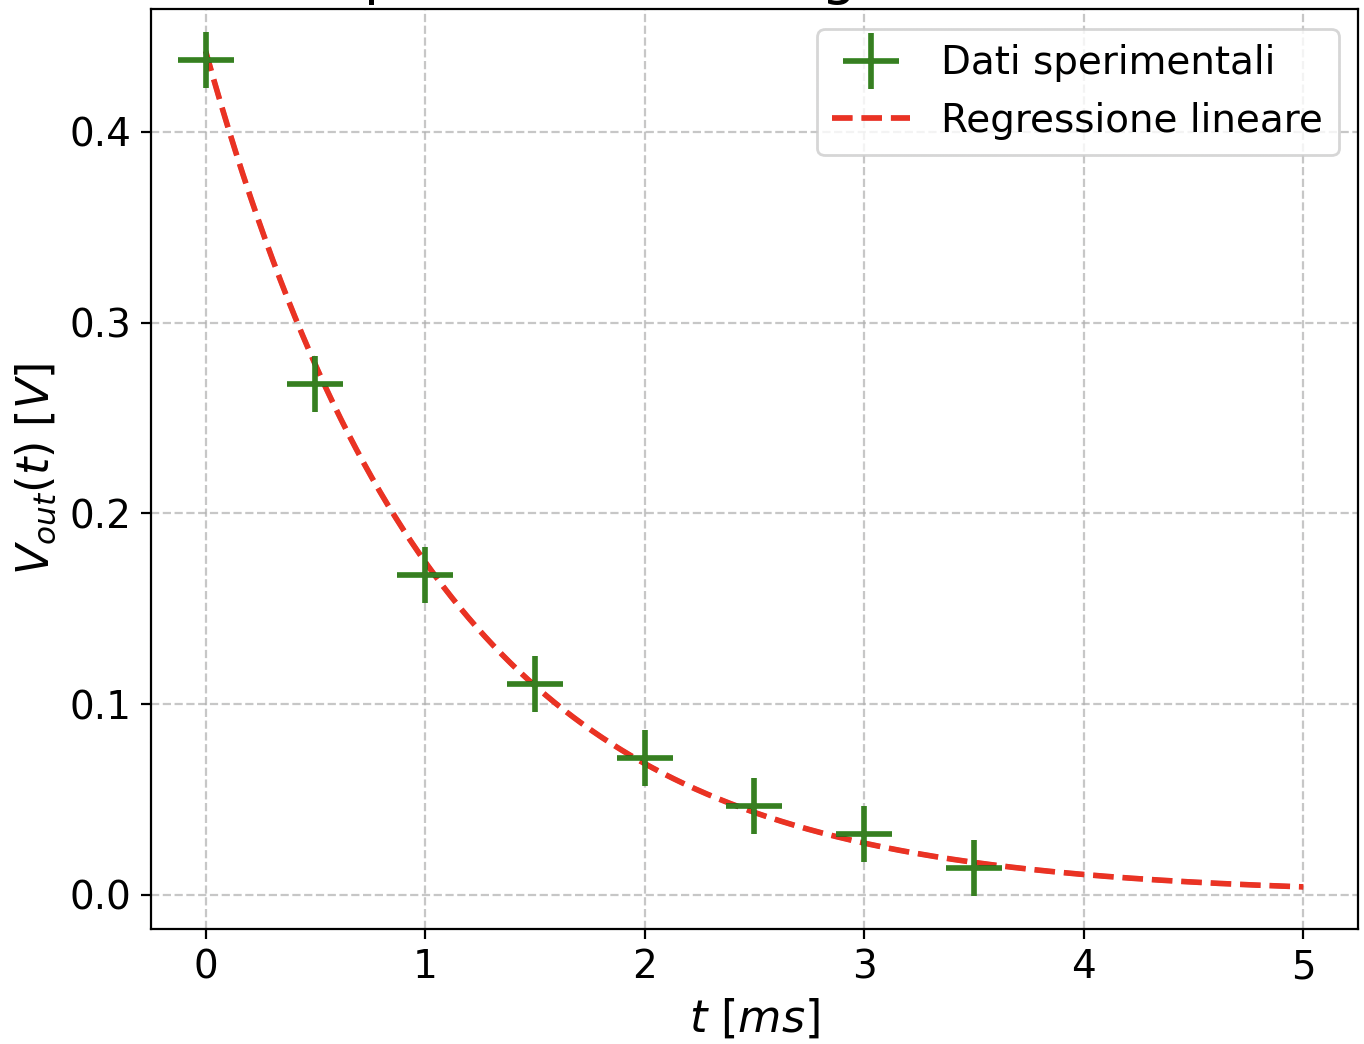
\includegraphics[width=0.5\linewidth]{es2.png}
    \caption{Regressione lineare sui dati sperimetali misurati}
    \label{fig:enter-label}
\end{figure}

Tramite il calcolo della regressione lineare è possibile determinare la costante di tempo del circuito utilizzando la risposta all’impulso, analizzando la fase di scarica del condensatore. La legge che descrive tale comportamento è, come visto prima, di tipo esponenziale, è quindi necessario applicare il logaritmo naturale a entrambi i membri dell’equazione, ottenendo una relazione lineare tra $\ln(V(t))$ e $t$:
$$\ln(V(t)) = \ln(V_0) - \frac{t}{\tau}$$
In questa forma, il termine $-1/\tau$ rappresenta la pendenza $m$ della retta, mentre $\ln(V_0)$ è l’intercetta $c$. La regressione lineare consente quindi di stimare i parametri $m$ e $c$, dai quali è possibile ricavare la costante di tempo $\tau = -1/m$.
Si calcola quindi  $\tau \approx 1 $$, \text{ms}$, in accordo con il valore teorico calcolato dai parametri del circuito.


%\section{ cosa fa rima con allegro }
%odio i froci
%odio i froci
%odio i froci
%odio i froci

\section{Esperimento 3: Diagramma ingresso-uscita circuito RC}
Nel seguente esercizio viene sempre preso in analisi il circuito precedente con \( R = 10 \, \text{k}\Omega \) e \( C = 100 \, \text{nF} \), avente però come segnale di ingresso una sinusoide di ampiezza picco-picco \( 5 \, \text{V} \) e offset pari a zero, variando per ogni misura la frequenza da un minimo di \( 1 \, \text{Hz} \) fino ad un massimo di \( 200 \, \text{kHz} \).

\begin{table}
    \centering
        \begin{tabular}{|c|c|c|c|}
        \hline
        Freq. & $\Delta x$ & $\Delta y$ & Sfasamento ($^\circ$) \\
        \hline
        1 Hz   & 0          & 0          & 0            \\
        2 Hz   & 0          & 0          & 0            \\
        5 Hz   & 0          & 40 mV      & 0            \\
        10 Hz  & 1 ms       & 60 mV      & 3.60          \\
        20 Hz  & 1.4 ms     & 120 mV     & 10.08        \\
        50 Hz  & 1.2 ms     & 240 mV     & 21.60         \\
        100 Hz & 1 ms       & 560 mV     & 36.00           \\
        200 Hz & 700 $\mu$s & 1.16 V     & 50.40         \\
        500 Hz & 390 $\mu$s & 1.90 V     & 70.20         \\
        1 kHz  & 226 $\mu$s & 2.17 V     & 81.36         \\
        2 kHz  & 116 $\mu$s & 2.33 V     & 83.52        \\
        5 kHz  & 46 $\mu$s  & 2.4 V      & 82.80         \\
        10 kHz & 24 $\mu$s  & 2.44 V     & 86.40         \\
        20 kHz & 12 $\mu$s  & 2.45 V     & 86.40         \\
        50 kHz & 4.6 $\mu$s & 2.47 V     & 82.80         \\
        100 kHz& 2.1 $\mu$s & 2.48 V     & 75.6         \\
        200 kHz& 400 ns     & 2.5 V      & 28.8         \\
        \hline
        \end{tabular}
    \caption{Tabella dei dati di frequenza, $\Delta x$, $\Delta y$ e    sfasamento in gradi.}
    \label{tab:dati_sfasamento}
\end{table}

Dai dati raccolti è possibile verificare il comportamento del circuito, secondo i quali inizialmente i segnali di ingresso e di uscita non sono sfasati e presentano una tensione di picco-picco simile. Successivamente aumentando la frequenza i due segnali si discostano tra di loro con uno sfasamento crescente e un valore di tensione decrescente per il segnale di uscita misurato sul condensatore. La fase tra i due segnali, misurata attraverso gli appositi cursori dell’oscilloscopio in ms, è stata convertita in gradi ° mediante la seguente formula:
$$\delta \degree= \delta [ms]T \cdot 360\degree$$
dove $\delta [ms]$ rappresenta lo sfasamento misurato e $T$ il periodo del segnale.
Per quanto riguarda il guadagno fornito dal circuito, esso è stato ricavato attraverso il rapporto tra uscita $Vin - \delta y$ e ingresso $Vin = 5 V$. 

\begin{figure}[h]
    \begin{minipage}{0.5\textwidth}   
        \centering
        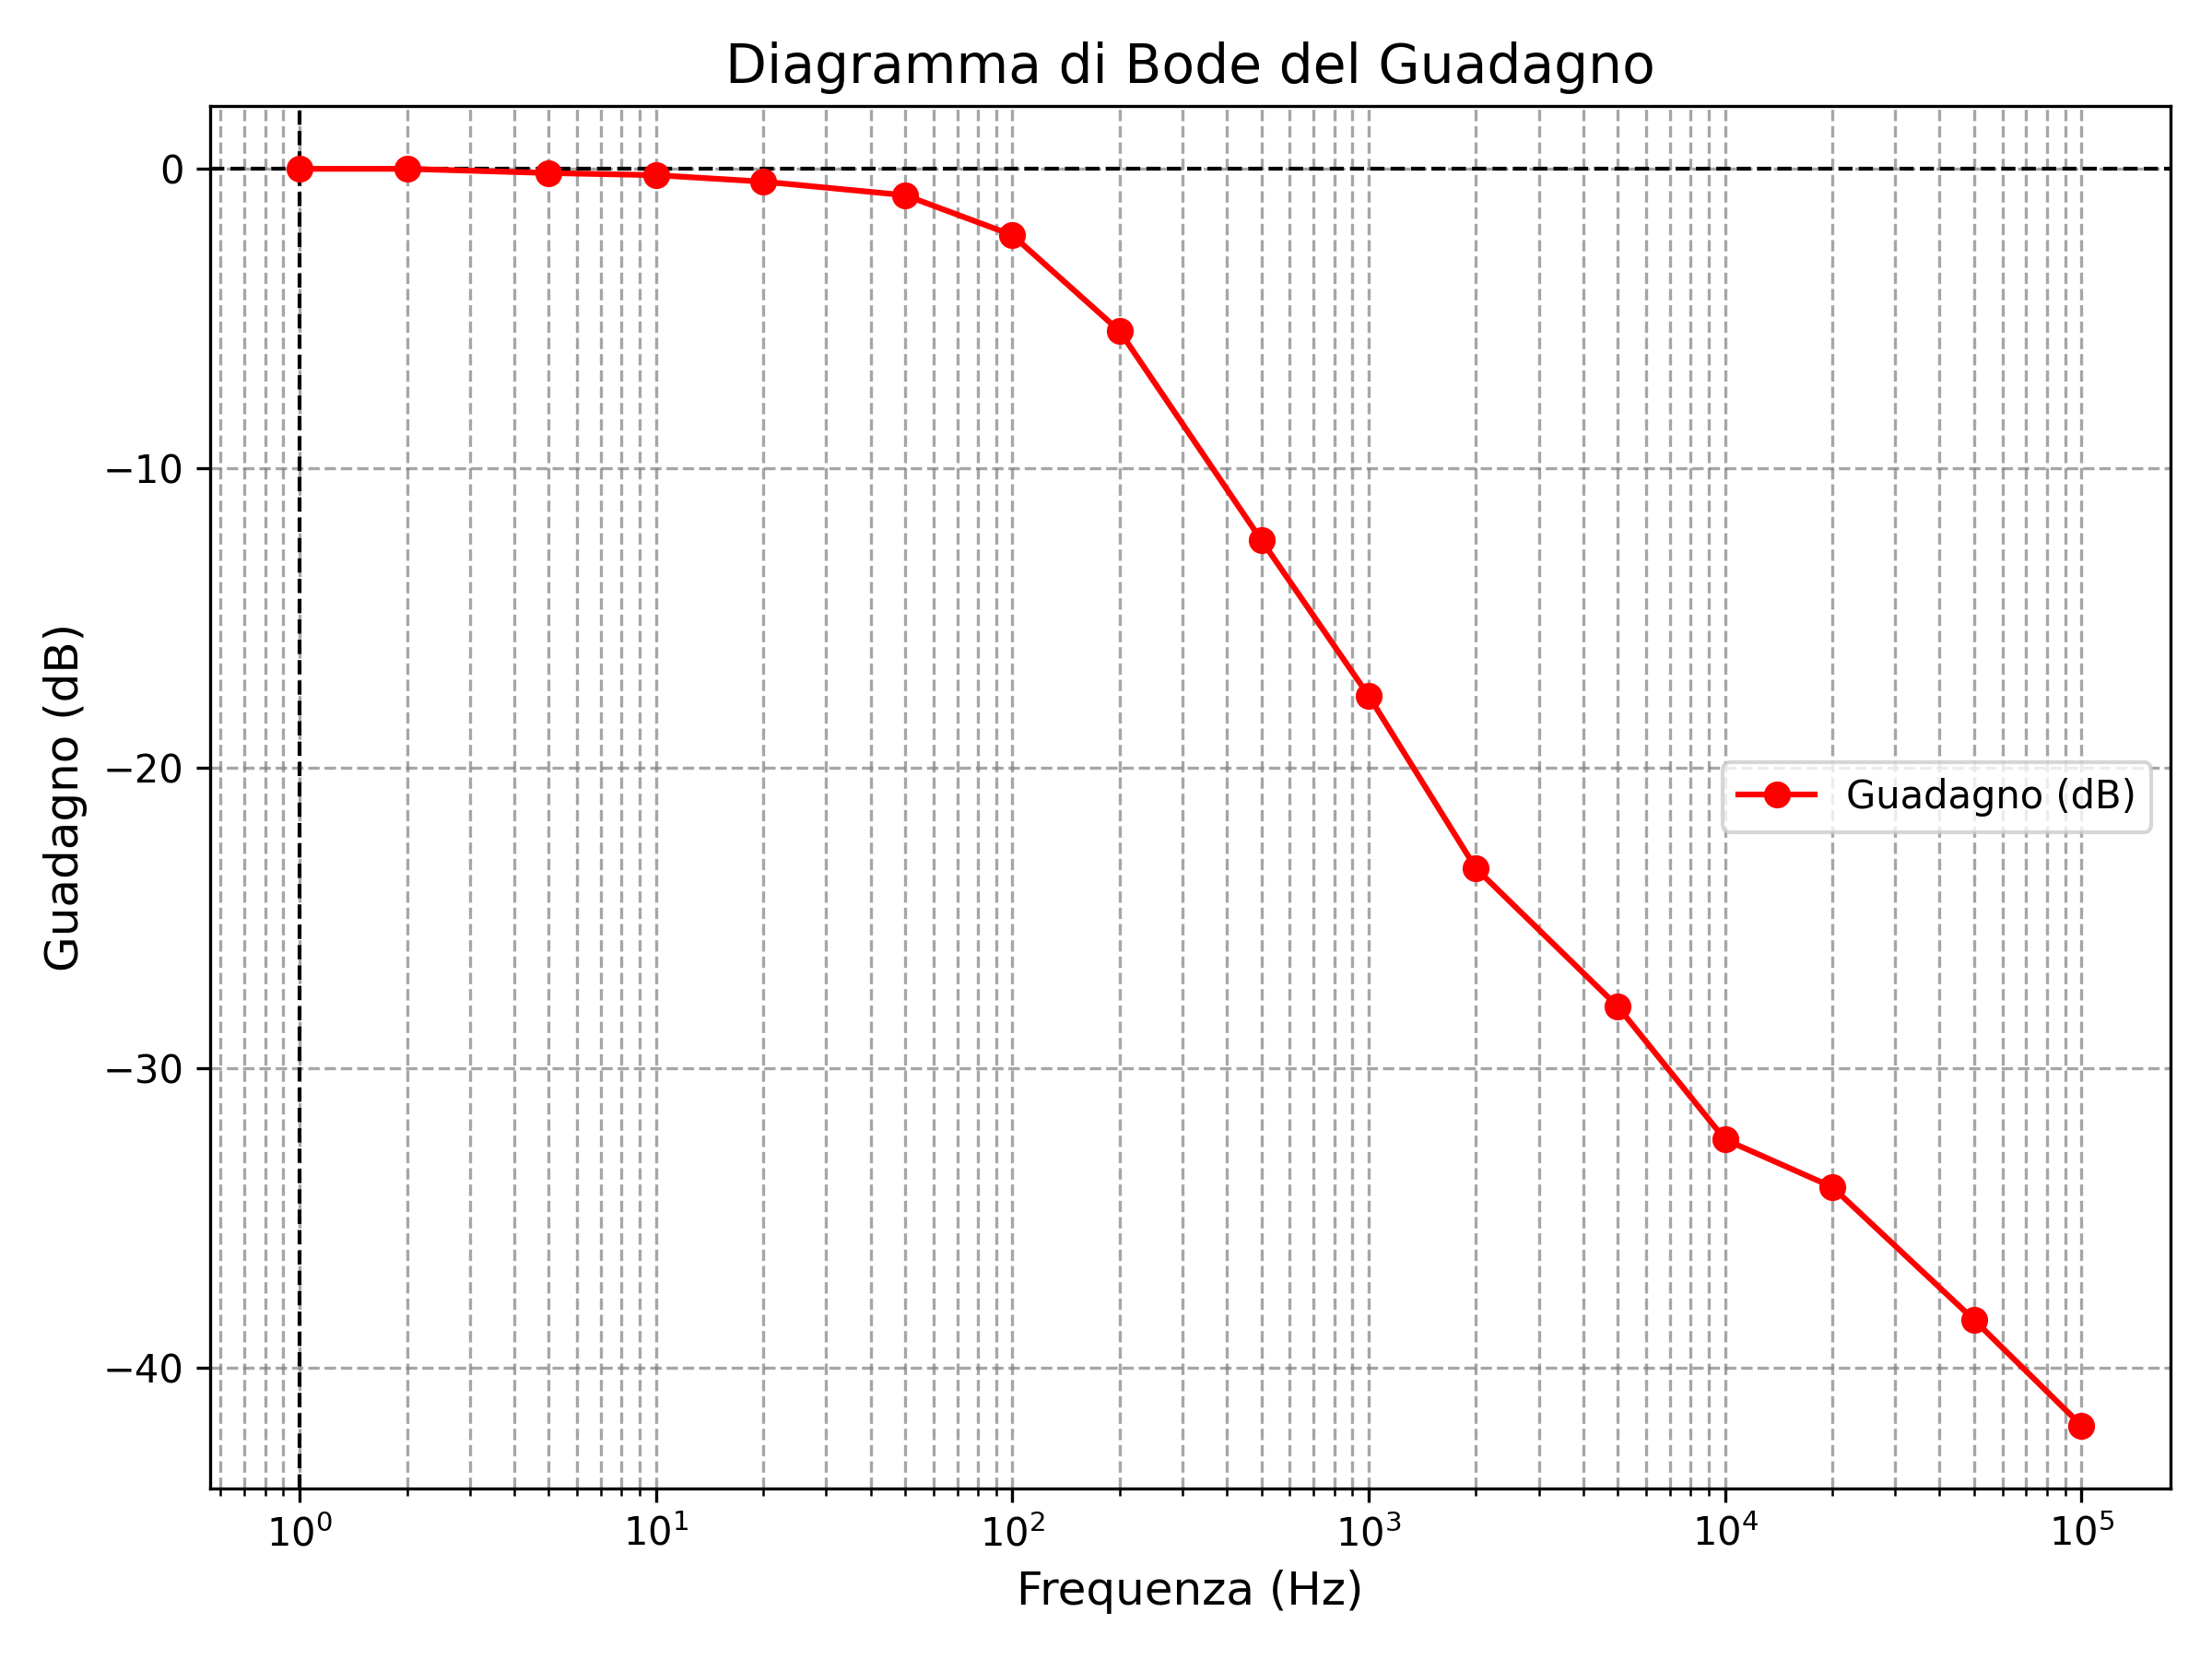
\includegraphics[width=0.8\linewidth]{guadagno_migliorato.png}
        \caption{Diagramma di Bode del guadagno}
        \label{fig:enter-label}
    \end{minipage}%
    \begin{minipage}{0.5\textwidth} 
        \centering
        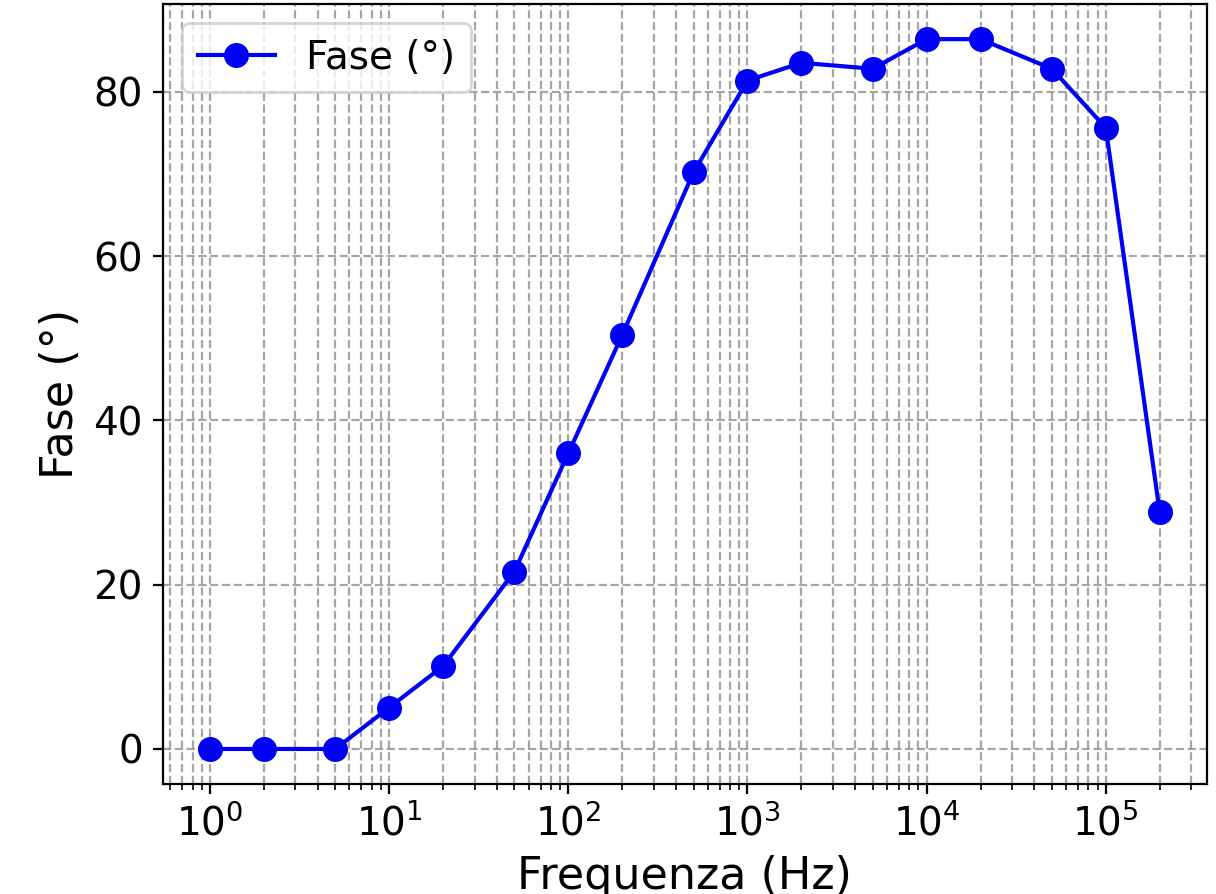
\includegraphics[width=0.8\linewidth]{fase_migliorato.png}
        \caption{Diagramma di Bode della fase}
        \label{fig:enter-label}
    \end{minipage}
\end{figure}


Per definire il funzionamento del circuito sono infine stati realizzati i diagrammi di Bode, in modo da rappresentare la sua risposta in frequenza, analizzandone modulo e fase attraverso i dati ottenuti sperimentalmente. Si nota come, per valori di frequenza inferiori rispetto a quella di taglio ($ft = 1/\tau = 1 KHz$, $f < 0.1ft$) il guadagno si aggira intorno a $1$ ($0$ in decibel), mentre per valori elevati ($f > 10ft$) esso tende a raggiungere il valore di $-20 dB$.  La conversione in decibel si esegue attraverso la seguente formula:

$$Av [dB]=20\log(Av)$$

Per quanto riguarda invece lo sfasamento, esso varia tra un massimo di $0$ e un minimo di $-90\degree$ (considerando opportunamente quale segnale precede l’altro, determinando così il segno della fase). In conclusione, l’andamento del circuito corrisponde a quello di un filtro passa basso RC, avente nei pressi della frequenza di taglio un modulo in decibel pari a circa $-3$ e una fase di $-45\degree$.
\end{document}